%%%%%%%%%%%%%%%%%%%%%%%%%%%%%%%%%%%%%%%%%
%  Sectioned Assignment
% LaTeX Template
% Version 1.0 (5/5/12)
%
% This template has been downloaded from:
% http://www.LaTeXTemplates.com
%
% Original author:
% Frits Wenneker (http://www.howtotex.com)
%
% License:
% CC BY-NC-SA 3.0 (http://creativecommons.org/licenses/by-nc-sa/3.0/)
%
%%%%%%%%%%%%%%%%%%%%%%%%%%%%%%%%%%%%%%%%%

%------------------------------------------------------------------------
%PACKAGES AND OTHER DOCUMENT CONFIGURATIONS
%------------------------------------------------------------------------

\documentclass[paper=a4, fontsize=11pt]{report} % A4 paper and 11pt font size

\usepackage[swedish, english]{babel} % Swedish and English language/hyphenation
\usepackage[T1]{fontenc} % Use 8-bit encoding that has 256 glyphs
\usepackage[a4paper]{geometry}
\usepackage{hyperref}
\usepackage[myheadings]{fullpage}
\usepackage{fancyhdr}
\usepackage{lastpage}
\usepackage{graphicx, wrapfig, subcaption, setspace, booktabs}
\usepackage[T1]{fontenc}
\usepackage[font=small, labelfont=bf]{caption}
\usepackage{fourier}
\usepackage[protrusion=true, expansion=true]{microtype}
\usepackage{sectsty}
\usepackage{url, lipsum}
\usepackage{amsmath}
\usepackage{float}
\usepackage{lmodern}
\usepackage[normalem]{ulem}
\useunder{\uline}{\ul}{}

%------------------------------------------------------------------------
%TITLE SECTION
%------------------------------------------------------------------------

\newcommand{\horrule}[1]{\rule{\linewidth}{#1}} % Create horizontal rule command with 1 argument of height
\onehalfspacing
\setcounter{tocdepth}{5}
\setcounter{secnumdepth}{5}
\usepackage{titlesec}

\pagestyle{fancy}
\fancyhf{}
\setlength\headheight{15pt}
\fancyhead[L]{Niklas Eliasson, Victor Persson}
\fancyhead[R]{Luleå Tekniska Universitet}
\fancyfoot[C]{\thepage}

\begin{document}

\title{
		\normalfont \normalsize
				\textsc{Luleå Tekniska Universitet} \\ [25pt] % Your university, school and/or department name(s)
				\horrule{1pt} \\[0.4cm] % top horizontal rule
				\huge Sprint 4 \\ % The assignment title
				\horrule{1pt} \\[0.5cm] % bottom horizontal rule
}

\author{Victor Persson,\\ Niklas Eliasson} % Your name

\date{\normalsize\today} % Today's date or a custom date

\maketitle % Print the title

\tableofcontents
\thispagestyle{empty}
\sectionfont{\scshape}
%
\newpage
\setcounter{page}{1}

%------------------------------------------------

\section*{Summary}
\addcontentsline{toc}{section}{Summary}
We are working on a e-comerce site for selling patches and accesories such as
belts and zippers for student overalls. It is intended to be dynamic with a
fully functional content management system. \\
			  For educational purposes Ruby on Rails was chosen. \\
			  Scrum planing was done at Trello.com and GitHub.com was used as VCS. \\


			  \section*{User stories}
			  \addcontentsline{toc}{section}{User stories}
			  Användare
			  \begin{itemize}
			  Sectioned\item Butiksadministratör
			  Sectioned\begin{itemize}
			  Assignment\item r/w priser
			  Assignment\item r/w kampanjer
			  Assignment\item r/w lagerstatus
			  Assignment\item r/w kategorier
			  Assignment\item r leveransstatus
			  Assignment\item r kundinfo
			  Sectioned\end{itemize}
			  Sectioned\item Lagerarbetare
			  Sectioned\begin{itemize}
			  Assignment\item r/w lagerstatus
			  Assignment\item r/w leveransstatus
			  Assignment\item r kundinfo
			  Sectioned\end{itemize}
			  Sectioned\item Inloggad kund
			  Sectioned\begin{itemize}
			  Assignment\item r/w sin egen kontaktinformation
		Assignment\item läsa sin egen orderhistorik
Assignment\item läsa sortimentet (produkter, priser, kampanjer, lagerstatus)
		Assignment\item lägga ordrar
		Assignment\item ? Spara/skicka kundkorg
		Sectioned\end{itemize}

		See Figure \ref{fig:2} - \ref{fig:4}

		\begin{figure}
		Sectioned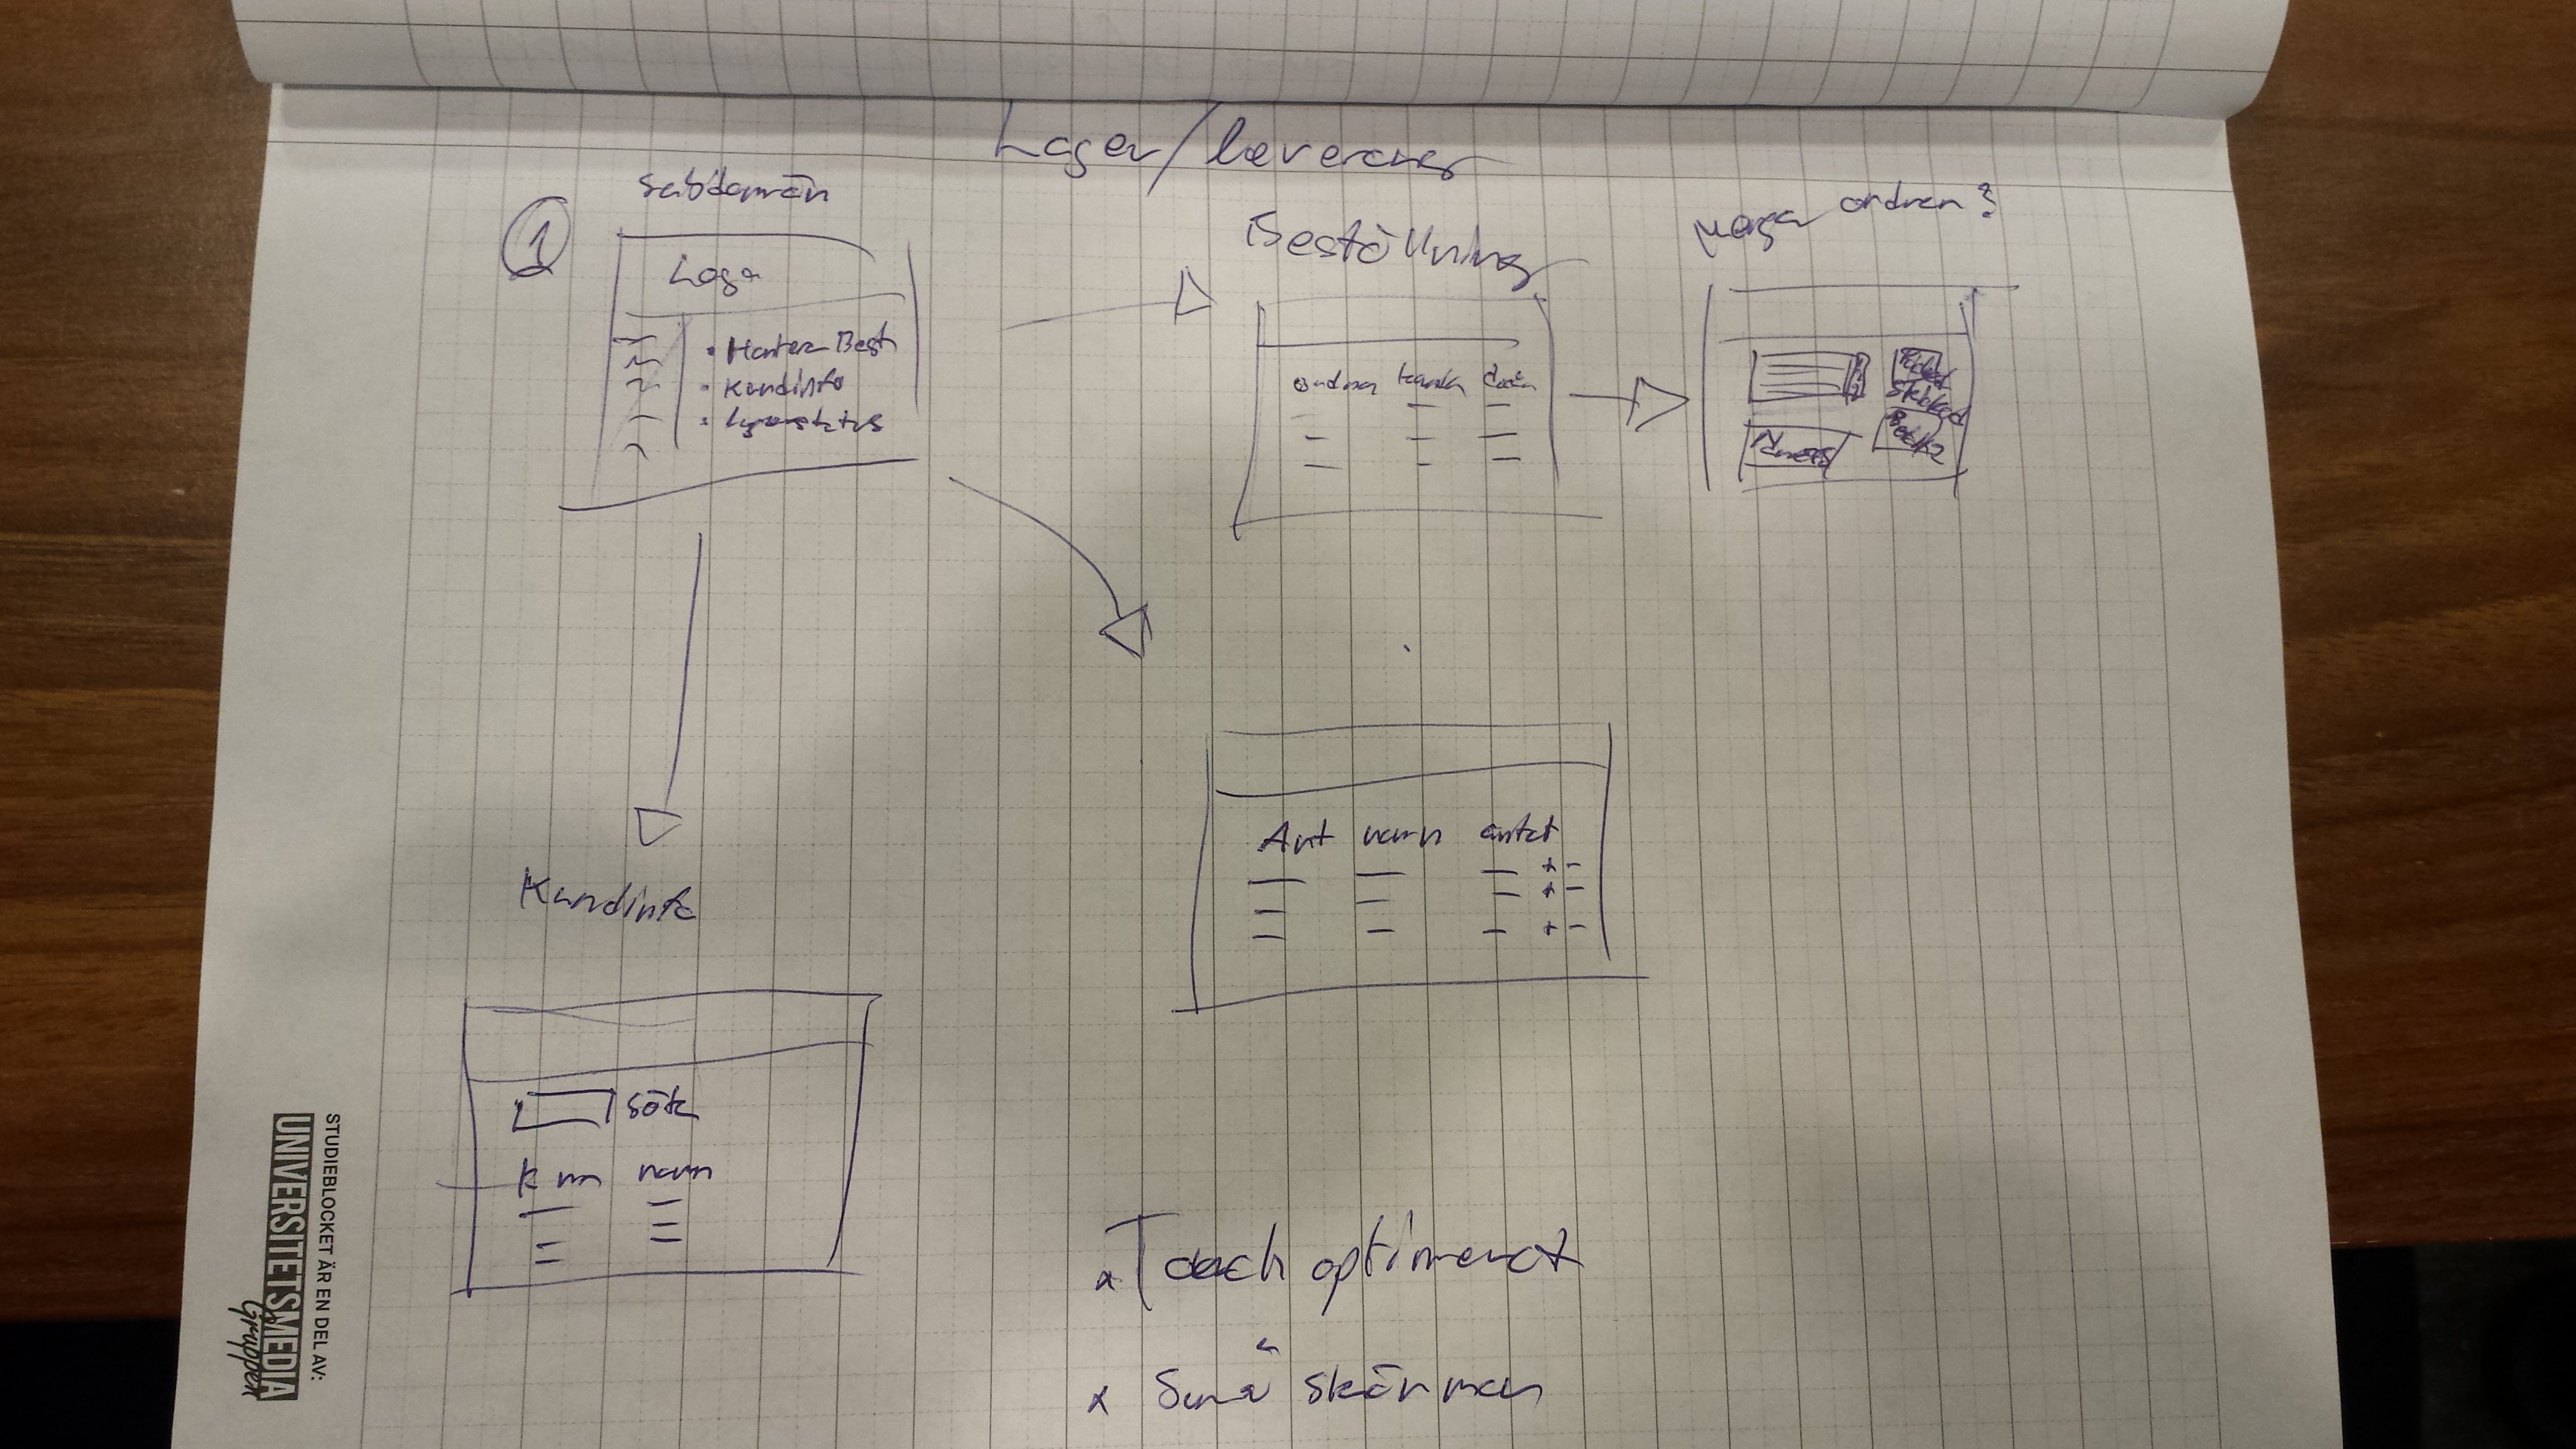
\includegraphics[scale=0.12]{artifacts/Lager.jpeg}
		Sectioned\caption{}
		Sectioned\label{fig:2}
		\end{figure}

		\begin{figure}
		Sectioned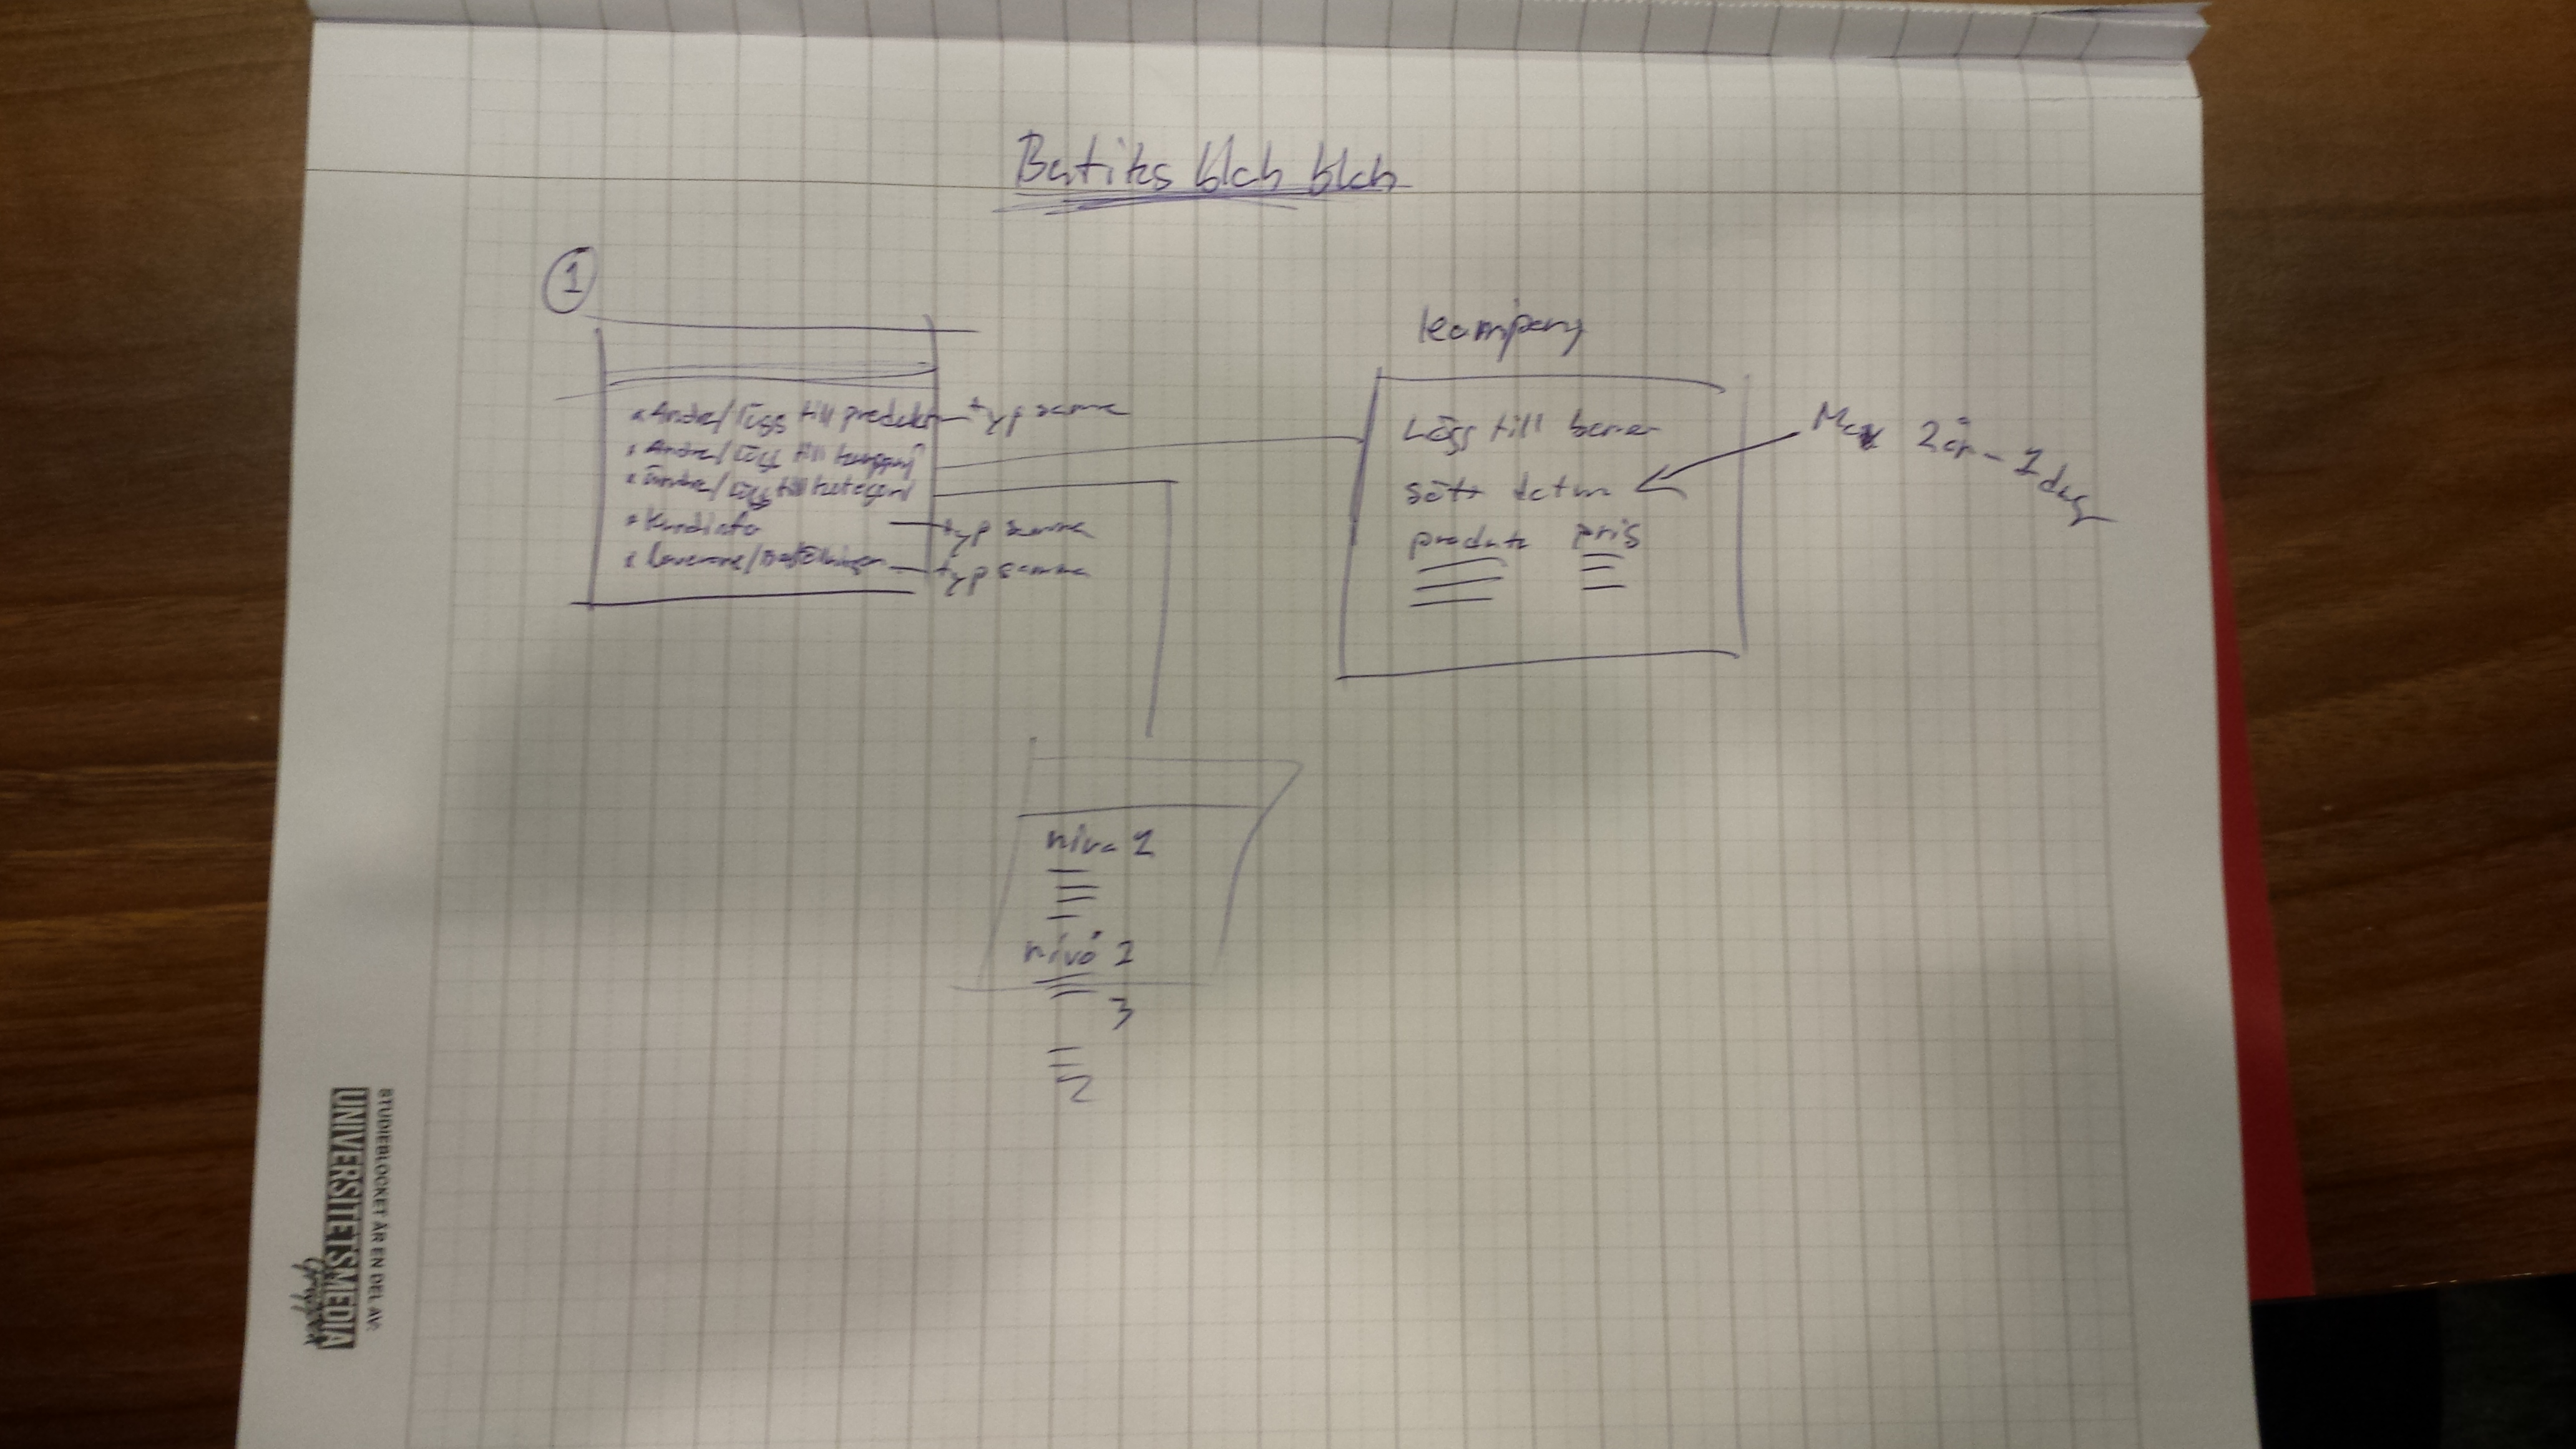
\includegraphics[scale=0.12]{artifacts/ButiksAdmin.jpeg}
		Sectioned\caption{}
		Sectioned\label{fig:3}
		\end{figure}

		\begin{figure}
		Sectioned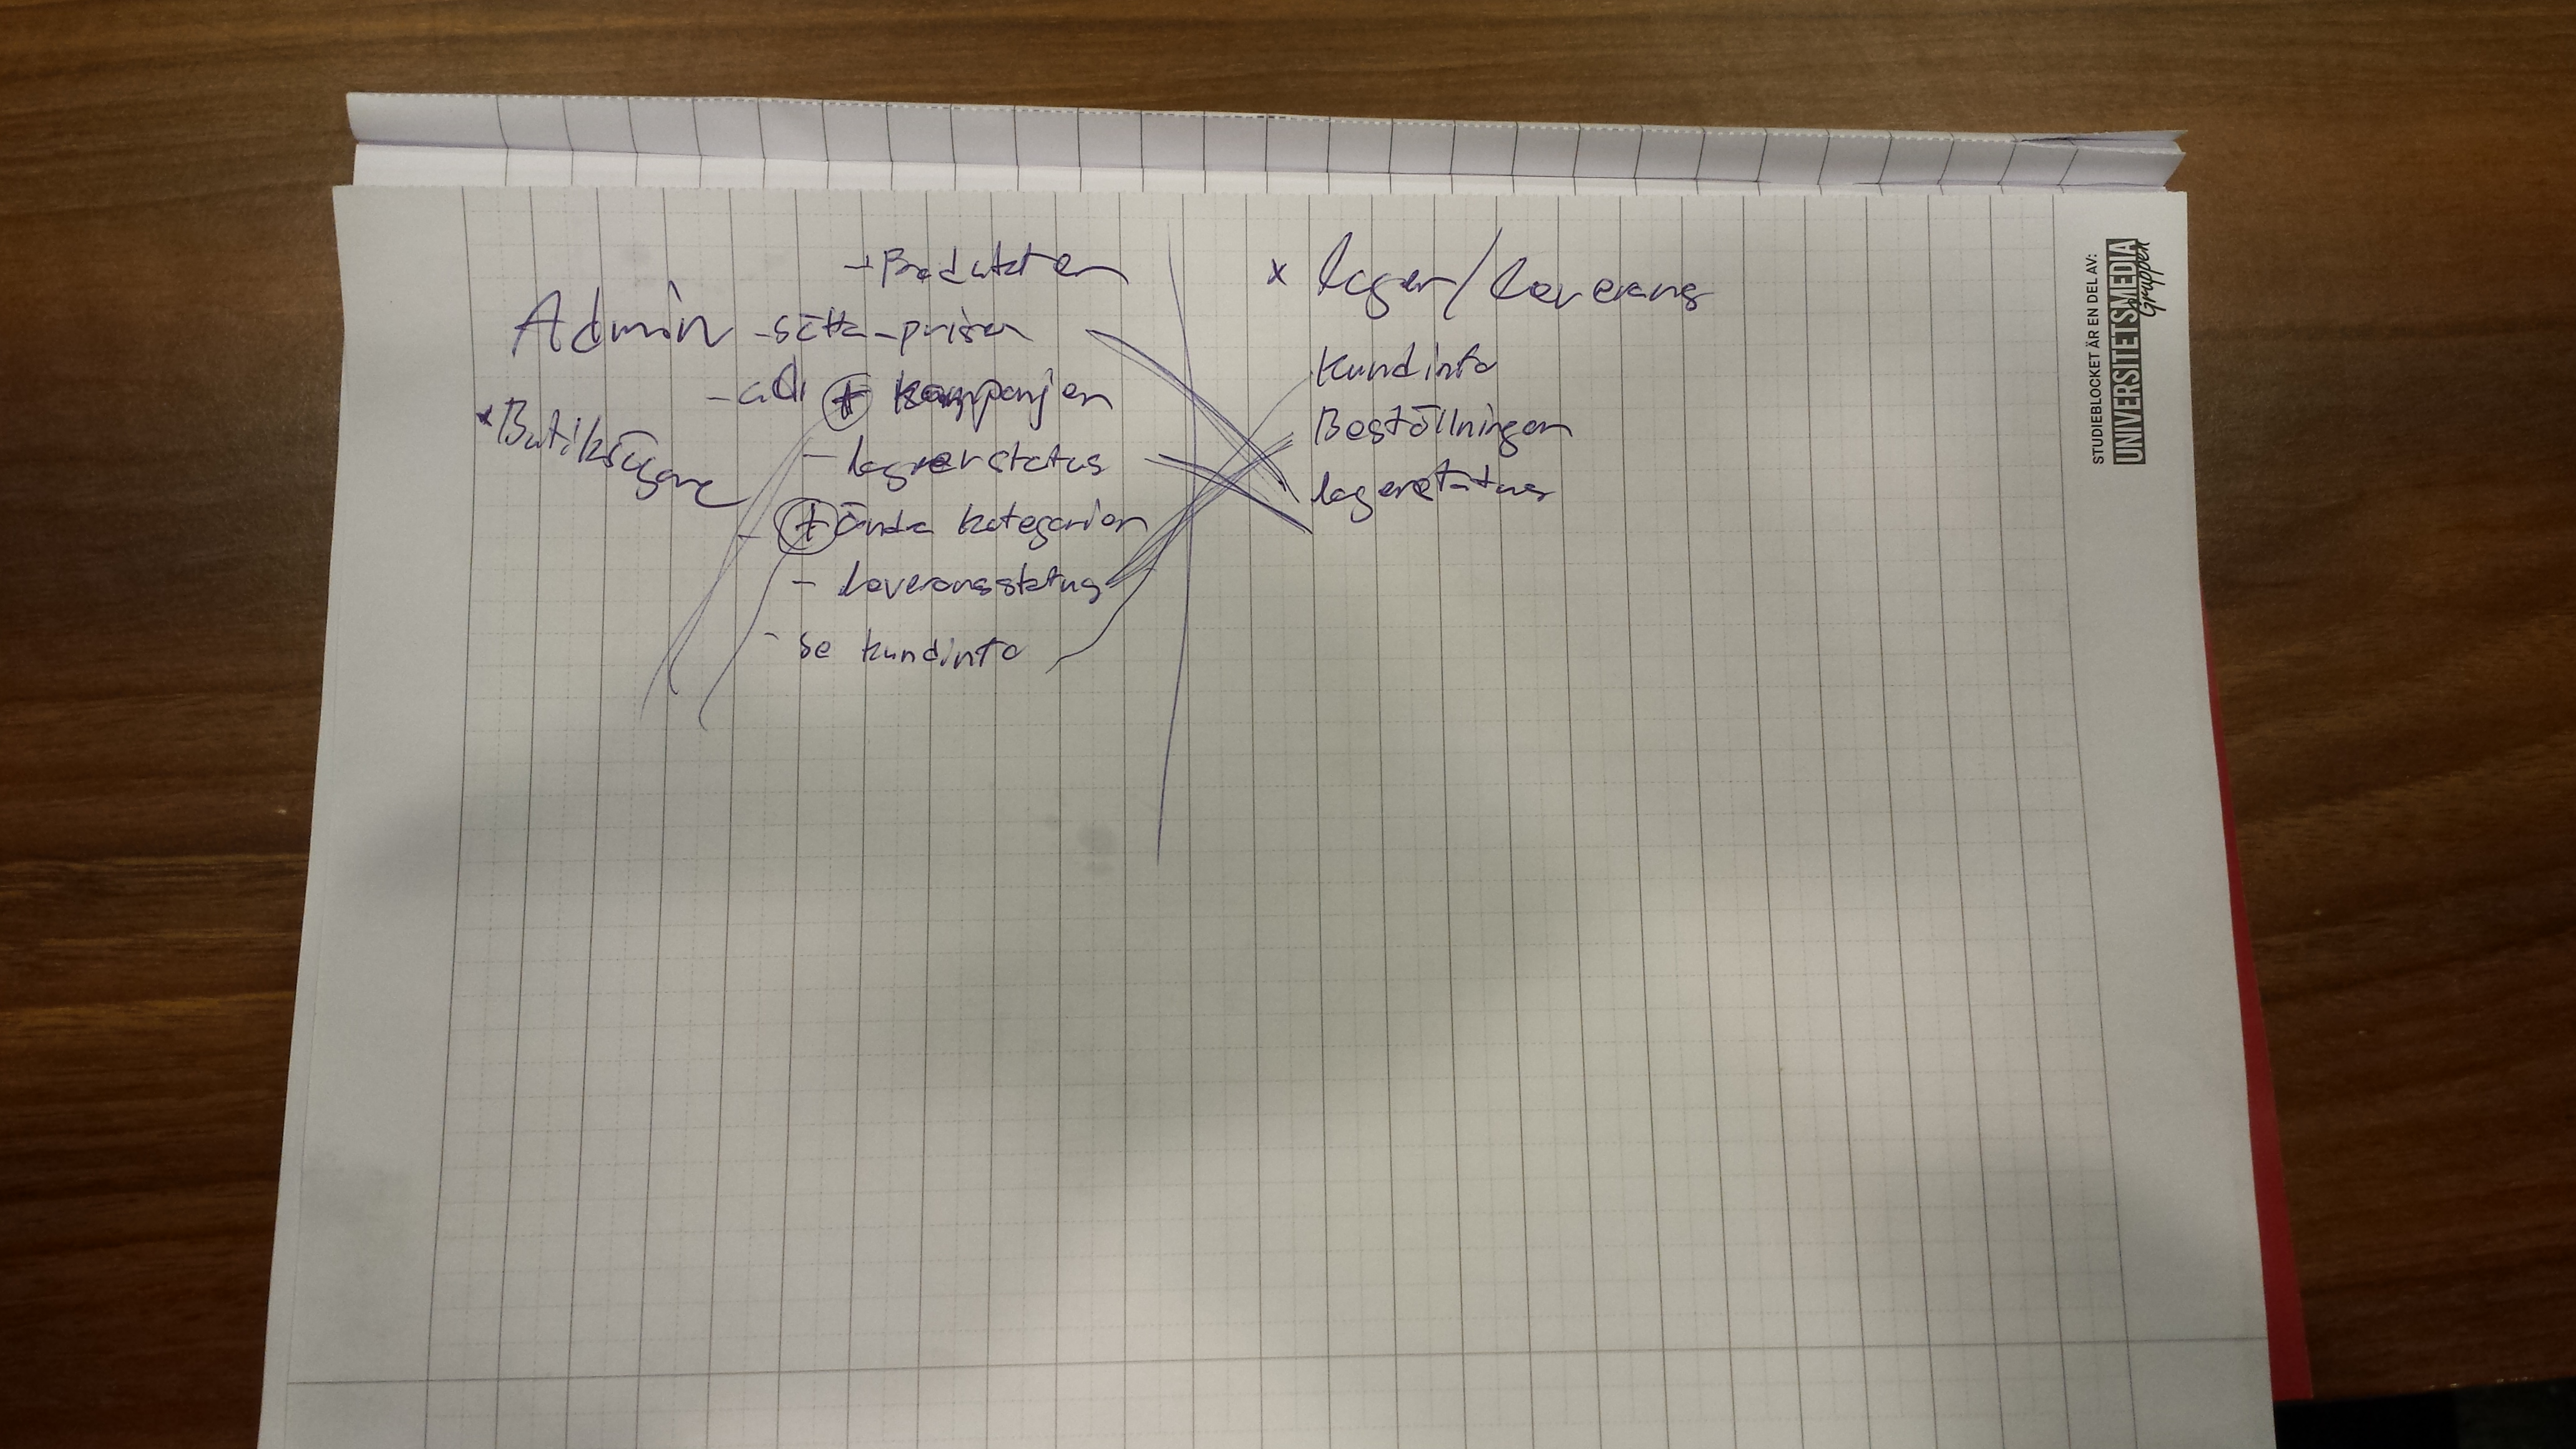
\includegraphics[scale=0.12]{artifacts/Admin.jpeg}
		Sectioned\caption{}
		Sectioned\label{fig:4}
		\end{figure}

		\section*{System architecture}
		\addcontentsline{toc}{section}{System architecture}
		During development we run the system on Ruby on Rails (RoR) built in web server
		Puma and sqlight3 for simplicity, but intend to move to a MariaDB database
		and a NGINX webserver with Phusion Passenger for RoR. We host
		the servers ourselves because it seemed seemed fun, educational and fairly simple.

		\section*{Backlog}
		\addcontentsline{toc}{section}{backlog}

		\begin{tabular}{|l|l|l|l|l|}
		Sectioned\hline
		Sectioned\#  & Sprint 4                      & Priority & Time est. & Description \\ \hline
		Sectioned301 & Startsida                     & 100      & 2         &             \\ \hline
		Sectioned302 & Dynamisk meny från kategorier & 90       & 2         &             \\ \hline
		Sectioned304 & Produktsida                   & 110      & 4         &             \\ \hline
		Sectioned305 & Kundkorg                      & 80       & 8         &             \\ \hline
		Sectioned307 & Profilsida (kundkort)         & 45       & 2         &             \\ \hline
		Sectioned308 & Orderhistorik                 & 45       & 1         &             \\ \hline
		Sectioned309 & Kundinlogg                    & 50       & 2         &             \\ \hline
		Sectioned310 & Registrering                  & 60       & 4         &             \\ \hline
		Sectioned312 & kommentarer/betygsättning     & 70       & 8         &             \\ \hline
		Sectioned313 & Produktkategorier             & 75       & 2         &             \\ \hline
		Sectioned400 & Backendinloggning             & 25       & 2         &             \\ \hline
		Sectioned1   & Personnummer -/+ hantering    & 5        & 1         &             \\ \hline
		\end{tabular}

		\begin{tabular}{|l|l|l|l|l|}
		Sectioned\hline
		Sectioned\#  & Left in backlog  & Priority & Time est. & Description \\ \hline
		Sectioned410 & Kampanjhantering & 10       & 3         &             \\ \hline
		Sectioned311 & Produktsökning   & 45       & 1         &             \\ \hline
		Sectioned306 & Betalsida        & 5        & 12        &             \\ \hline


		Planing is done at Trello.com
		\url{https://trello.com/b/JxDCHBcm}\
				This is just a small section of the backlog. For history of all sprints and deeper
				explanation of the backlog items, refer to Trello.

				\section*{Database schema}
				\addcontentsline{toc}{section}{Database schema}
				See Figure \ref{fig:6}
				\begin{figure}
				Sectioned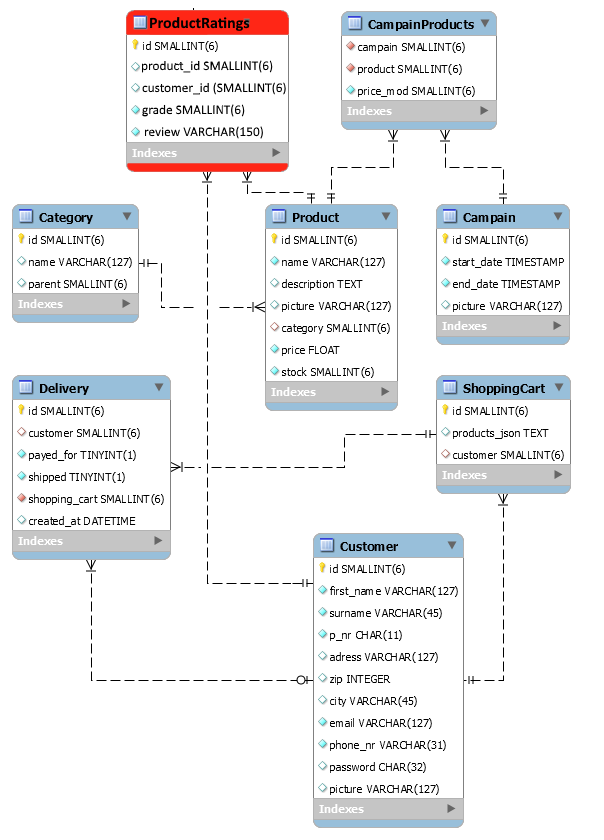
\includegraphics[scale=0.7]{artifacts/db_implemented_1_3.png}
				Sectioned\caption{Database design.}
				Sectioned\label{fig:6}
				\end{figure}

				\section*{Code}
				\addcontentsline{toc}{section}{Code}
				All code is avalible at github.
				\url{https://github.com/nikalas/D0018E-Databasteknik.git}

				\section*{Test case specifications}
				\addcontentsline{toc}{section}{Test case specifications}

Problem: Item out of stock? \
				A customer adds a product to the basket. If the product goes out of
				stock before checkout, how is this handled?

				Solution: \
						At checkout a check is made if the product is still in stock. If not
						the custumer is brought back to the 'carts' page and asked to remove
						the product that is no longer available and that the cart has to be
						updated.

						\section*{Limitations and improvements}
						\addcontentsline{toc}{section}{Limitations and improvements}

						We decided to put off saving payment methods and/or information. Might
						end up readding it to the backlog if it looks like we will have time
						to spare. Non-registerd customers have also been put on hold for now.
						Products search, sorting, sale campaigns, and uploading pictures
						through the backend has also been put on hold, since we didn't have
						time to fully implement them.

						\end{document}
